% =====================================================================
%  SLIDES (Beamer/metropolis) — CSRF on Elgg with the Fetch API (English)
%  Build: xelatex slides_en.tex  (run twice)
% =====================================================================
\documentclass[11pt,aspectratio=169]{beamer}
\usetheme{metropolis}
\metroset{progressbar=frametitle,numbering=fraction,block=fill,sectionpage=none}

\usepackage{fontspec}
\setsansfont{TeX Gyre Heros}
\setmonofont{Noto Sans Mono}[Scale=0.82]
\usepackage[english]{babel}

% ---- Brand colours ----
\definecolor{navy}{HTML}{1E3C72}
\definecolor{brandblue}{HTML}{2A5298}
\definecolor{accent}{HTML}{2563EB}
\definecolor{danger}{HTML}{DC2626}
\definecolor{success}{HTML}{15803D}
\definecolor{amber}{HTML}{B45309}
\definecolor{slate}{HTML}{475569}
\definecolor{ink}{HTML}{0F172A}
\definecolor{mist}{HTML}{F1F5F9}
\setbeamercolor{frametitle}{bg=navy}
\setbeamercolor{progress bar}{fg=accent,bg=mist}
\setbeamercolor{title separator}{fg=accent}
\setbeamercolor{alerted text}{fg=danger}
\setbeamercolor{block title}{bg=brandblue,fg=white}
\setbeamercolor{block body}{bg=mist}
\setbeamercolor{block title alerted}{bg=danger,fg=white}
\setbeamercolor{block body alerted}{bg=danger!8,fg=black}
\setbeamercolor{block title example}{bg=success,fg=white}
\setbeamercolor{block body example}{bg=success!8,fg=black}

\usepackage{tikz}
\usetikzlibrary{arrows.meta,positioning,calc}
\usepackage{booktabs}
\usepackage{graphicx}
\usepackage{listings}
\definecolor{codebg}{HTML}{0F172A}\definecolor{codefg}{HTML}{E2E8F0}
\definecolor{codekey}{HTML}{38BDF8}\definecolor{codestr}{HTML}{86EFAC}
\definecolor{codecom}{HTML}{94A3B8}\definecolor{line}{HTML}{CBD5E1}
\lstset{basicstyle=\scriptsize\ttfamily\color{codefg},backgroundcolor=\color{codebg},
  keywordstyle=\color{codekey}\bfseries,stringstyle=\color{codestr},
  commentstyle=\color{codecom}\itshape,frame=single,framerule=0pt,
  rulecolor=\color{codebg},showstringspaces=false,breaklines=true,
  columns=fullflexible,keepspaces=true,xleftmargin=8pt,aboveskip=4pt,belowskip=2pt}
\lstdefinelanguage{JS}{keywords={const,let,new,async,await,fetch,return,function},
  morekeywords=[2]{URLSearchParams,FormData,append,addEventListener},
  keywordstyle=[2]\color{codestr}\bfseries,sensitive=true,
  morecomment=[l]{//},morestring=[b]',morestring=[b]"}
\usepackage{pifont}
\newcommand{\yes}{\textcolor{success}{\ding{52}}}
\newcommand{\no}{\textcolor{danger}{\ding{56}}}

% ---- diagram (English labels) ----
\providecommand{\lblVictim}{Alice (victim) + Browser}
\providecommand{\lblAttacker}{Attacker\\\texttt{attacker.csrf.localhost}}
\providecommand{\lblElgg}{Elgg\\\texttt{elgg.csrf.localhost}}
\providecommand{\lblSa}{1. Legitimate login}
\providecommand{\lblSb}{2. Set-Cookie \texttt{Elgg=...}}
\providecommand{\lblSc}{3. Victim opens malicious page}
\providecommand{\lblSd}{4. Returns \texttt{index.html} (Fetch script)}
\providecommand{\lblNe}{5. Script auto-runs (\texttt{DOMContentLoaded})}
\providecommand{\lblSf}{6. Fetch POST + cookie (\texttt{credentials:'include'})}
\providecommand{\lblNg}{7. Valid cookie $\Rightarrow$ About me updated}
\providecommand{\lblSh}{8. Response 302 (opaque)}
\providecommand{\lblSi}{9. Reload profile $\to$ changed}
% =====================================================================
%  diagram_flow.tex — CSRF attack sequence diagram (\csrfflowdiagram)
%  Labels default to Vietnamese; an English document may \renewcommand
%  them BEFORE % =====================================================================
%  diagram_flow.tex — CSRF attack sequence diagram (\csrfflowdiagram)
%  Labels default to Vietnamese; an English document may \renewcommand
%  them BEFORE % =====================================================================
%  diagram_flow.tex — CSRF attack sequence diagram (\csrfflowdiagram)
%  Labels default to Vietnamese; an English document may \renewcommand
%  them BEFORE \input{diagram_flow}.
% =====================================================================
\providecommand{\lblVictim}{Alice (nạn nhân) + Trình duyệt}
\providecommand{\lblAttacker}{Attacker\\\texttt{attacker32.com}}
\providecommand{\lblElgg}{Elgg\\\texttt{seed-server.com}}
\providecommand{\lblSa}{1. Đăng nhập hợp lệ}
\providecommand{\lblSb}{2. Set-Cookie \texttt{Elgg=...}}
\providecommand{\lblSc}{3. Vô tình mở trang độc hại}
\providecommand{\lblSd}{4. Trả \texttt{index.html} (Fetch script)}
\providecommand{\lblNe}{5. Script tự chạy (\texttt{DOMContentLoaded})}
\providecommand{\lblSf}{6. Fetch POST + cookie (\texttt{credentials:'include'})}
\providecommand{\lblNg}{7. Cookie hợp lệ $\Rightarrow$ cập nhật About me}
\providecommand{\lblSh}{8. Phản hồi 302 (opaque)}
\providecommand{\lblSi}{9. Xem lại hồ sơ $\to$ đã bị đổi}

\newcommand{\csrfflowdiagram}{%
\begin{tikzpicture}[
   >={Stealth[length=2.4mm]}, font=\sffamily\scriptsize,
   head/.style={draw=navy,fill=navy,text=white,rounded corners=3pt,
                align=center,minimum height=0.85cm,minimum width=3.2cm,
                font=\sffamily\scriptsize\bfseries},
   life/.style={line,dashed,line width=0.7pt},
   msg/.style={->,accent,line width=0.9pt},
   ret/.style={->,slate,line width=0.7pt,dashed},
   note/.style={draw=amber,fill=amber!12,rounded corners=2pt,align=center,
                inner sep=3pt,font=\sffamily\scriptsize,text=amber!60!black}]

  \def\ax{0} \def\bx{5.4} \def\cx{10.8}
  \def\ytop{0} \def\ybot{-9.3}

  % lifeline heads
  \node[head] (A) at (\ax,\ytop) {\lblVictim};
  \node[head] (B) at (\bx,\ytop) {\lblAttacker};
  \node[head] (C) at (\cx,\ytop) {\lblElgg};

  % lifelines
  \draw[life] (\ax,-0.55) -- (\ax,\ybot);
  \draw[life] (\bx,-0.55) -- (\bx,\ybot);
  \draw[life] (\cx,-0.55) -- (\cx,\ybot);

  % messages
  \draw[msg] (\ax,-1.2) -- node[above]{\lblSa} (\cx,-1.2);
  \draw[ret] (\cx,-2.0) -- node[above]{\lblSb} (\ax,-2.0);
  \draw[msg] (\ax,-2.9) -- node[above]{\lblSc} (\bx,-2.9);
  \draw[ret] (\bx,-3.7) -- node[above]{\lblSd} (\ax,-3.7);

  \node[note,anchor=north west] at (\ax-1.7,-4.35) {\lblNe};

  \draw[msg,danger] (\ax,-5.6) -- node[above,text=danger]{\lblSf} (\cx,-5.6);

  \node[note,anchor=north] at (\cx,-6.2) {\lblNg};

  \draw[ret] (\cx,-7.4) -- node[above]{\lblSh} (\ax,-7.4);
  \draw[msg,success] (\ax,-8.4) -- node[above,text=success]{\lblSi} (\cx,-8.4);
\end{tikzpicture}%
}
.
% =====================================================================
\providecommand{\lblVictim}{Alice (nạn nhân) + Trình duyệt}
\providecommand{\lblAttacker}{Attacker\\\texttt{attacker32.com}}
\providecommand{\lblElgg}{Elgg\\\texttt{seed-server.com}}
\providecommand{\lblSa}{1. Đăng nhập hợp lệ}
\providecommand{\lblSb}{2. Set-Cookie \texttt{Elgg=...}}
\providecommand{\lblSc}{3. Vô tình mở trang độc hại}
\providecommand{\lblSd}{4. Trả \texttt{index.html} (Fetch script)}
\providecommand{\lblNe}{5. Script tự chạy (\texttt{DOMContentLoaded})}
\providecommand{\lblSf}{6. Fetch POST + cookie (\texttt{credentials:'include'})}
\providecommand{\lblNg}{7. Cookie hợp lệ $\Rightarrow$ cập nhật About me}
\providecommand{\lblSh}{8. Phản hồi 302 (opaque)}
\providecommand{\lblSi}{9. Xem lại hồ sơ $\to$ đã bị đổi}

\newcommand{\csrfflowdiagram}{%
\begin{tikzpicture}[
   >={Stealth[length=2.4mm]}, font=\sffamily\scriptsize,
   head/.style={draw=navy,fill=navy,text=white,rounded corners=3pt,
                align=center,minimum height=0.85cm,minimum width=3.2cm,
                font=\sffamily\scriptsize\bfseries},
   life/.style={line,dashed,line width=0.7pt},
   msg/.style={->,accent,line width=0.9pt},
   ret/.style={->,slate,line width=0.7pt,dashed},
   note/.style={draw=amber,fill=amber!12,rounded corners=2pt,align=center,
                inner sep=3pt,font=\sffamily\scriptsize,text=amber!60!black}]

  \def\ax{0} \def\bx{5.4} \def\cx{10.8}
  \def\ytop{0} \def\ybot{-9.3}

  % lifeline heads
  \node[head] (A) at (\ax,\ytop) {\lblVictim};
  \node[head] (B) at (\bx,\ytop) {\lblAttacker};
  \node[head] (C) at (\cx,\ytop) {\lblElgg};

  % lifelines
  \draw[life] (\ax,-0.55) -- (\ax,\ybot);
  \draw[life] (\bx,-0.55) -- (\bx,\ybot);
  \draw[life] (\cx,-0.55) -- (\cx,\ybot);

  % messages
  \draw[msg] (\ax,-1.2) -- node[above]{\lblSa} (\cx,-1.2);
  \draw[ret] (\cx,-2.0) -- node[above]{\lblSb} (\ax,-2.0);
  \draw[msg] (\ax,-2.9) -- node[above]{\lblSc} (\bx,-2.9);
  \draw[ret] (\bx,-3.7) -- node[above]{\lblSd} (\ax,-3.7);

  \node[note,anchor=north west] at (\ax-1.7,-4.35) {\lblNe};

  \draw[msg,danger] (\ax,-5.6) -- node[above,text=danger]{\lblSf} (\cx,-5.6);

  \node[note,anchor=north] at (\cx,-6.2) {\lblNg};

  \draw[ret] (\cx,-7.4) -- node[above]{\lblSh} (\ax,-7.4);
  \draw[msg,success] (\ax,-8.4) -- node[above,text=success]{\lblSi} (\cx,-8.4);
\end{tikzpicture}%
}
.
% =====================================================================
\providecommand{\lblVictim}{Alice (nạn nhân) + Trình duyệt}
\providecommand{\lblAttacker}{Attacker\\\texttt{attacker32.com}}
\providecommand{\lblElgg}{Elgg\\\texttt{seed-server.com}}
\providecommand{\lblSa}{1. Đăng nhập hợp lệ}
\providecommand{\lblSb}{2. Set-Cookie \texttt{Elgg=...}}
\providecommand{\lblSc}{3. Vô tình mở trang độc hại}
\providecommand{\lblSd}{4. Trả \texttt{index.html} (Fetch script)}
\providecommand{\lblNe}{5. Script tự chạy (\texttt{DOMContentLoaded})}
\providecommand{\lblSf}{6. Fetch POST + cookie (\texttt{credentials:'include'})}
\providecommand{\lblNg}{7. Cookie hợp lệ $\Rightarrow$ cập nhật About me}
\providecommand{\lblSh}{8. Phản hồi 302 (opaque)}
\providecommand{\lblSi}{9. Xem lại hồ sơ $\to$ đã bị đổi}

\newcommand{\csrfflowdiagram}{%
\begin{tikzpicture}[
   >={Stealth[length=2.4mm]}, font=\sffamily\scriptsize,
   head/.style={draw=navy,fill=navy,text=white,rounded corners=3pt,
                align=center,minimum height=0.85cm,minimum width=3.2cm,
                font=\sffamily\scriptsize\bfseries},
   life/.style={line,dashed,line width=0.7pt},
   msg/.style={->,accent,line width=0.9pt},
   ret/.style={->,slate,line width=0.7pt,dashed},
   note/.style={draw=amber,fill=amber!12,rounded corners=2pt,align=center,
                inner sep=3pt,font=\sffamily\scriptsize,text=amber!60!black}]

  \def\ax{0} \def\bx{5.4} \def\cx{10.8}
  \def\ytop{0} \def\ybot{-9.3}

  % lifeline heads
  \node[head] (A) at (\ax,\ytop) {\lblVictim};
  \node[head] (B) at (\bx,\ytop) {\lblAttacker};
  \node[head] (C) at (\cx,\ytop) {\lblElgg};

  % lifelines
  \draw[life] (\ax,-0.55) -- (\ax,\ybot);
  \draw[life] (\bx,-0.55) -- (\bx,\ybot);
  \draw[life] (\cx,-0.55) -- (\cx,\ybot);

  % messages
  \draw[msg] (\ax,-1.2) -- node[above]{\lblSa} (\cx,-1.2);
  \draw[ret] (\cx,-2.0) -- node[above]{\lblSb} (\ax,-2.0);
  \draw[msg] (\ax,-2.9) -- node[above]{\lblSc} (\bx,-2.9);
  \draw[ret] (\bx,-3.7) -- node[above]{\lblSd} (\ax,-3.7);

  \node[note,anchor=north west] at (\ax-1.7,-4.35) {\lblNe};

  \draw[msg,danger] (\ax,-5.6) -- node[above,text=danger]{\lblSf} (\cx,-5.6);

  \node[note,anchor=north] at (\cx,-6.2) {\lblNg};

  \draw[ret] (\cx,-7.4) -- node[above]{\lblSh} (\ax,-7.4);
  \draw[msg,success] (\ax,-8.4) -- node[above,text=success]{\lblSi} (\cx,-8.4);
\end{tikzpicture}%
}


% ---- Title metadata ----
\title{Cross-Site Request Forgery on Elgg via the Fetch API}
\subtitle{Replacing XMLHttpRequest / form submit with modern \texttt{fetch()}}
\author{Group 6 — Thanh (23001935) · Tri (23001939) · Thao (23001936)}
\institute{Computer Security — VNU University of Science}
\date{\today}

\begin{document}

{\setbeamercolor{background canvas}{bg=navy}
\setbeamercolor{normal text}{fg=white}
\setbeamercolor{title}{fg=white}\setbeamercolor{subtitle}{fg=mist}
\setbeamercolor{author}{fg=mist}\setbeamercolor{institute}{fg=mist}\setbeamercolor{date}{fg=mist}
\begin{frame}[plain]\titlepage\end{frame}}

% ---------------------------------------------------------------
\begin{frame}{Outline \& responsibilities}
  \begin{columns}[t]
    \column{0.52\textwidth}
      \setbeamertemplate{section in toc}[sections numbered]
      \tableofcontents
    \column{0.46\textwidth}
      \footnotesize
      \textbf{Responsibilities (Group 6):}
      \begin{itemize}\footnotesize
        \item \textbf{Thanh} — theory, HTTP, defenses
        \item \textbf{Tri} — Elgg, Docker, Fetch API, testing
        \item \textbf{Thao} — evidence, slides, video
      \end{itemize}
      \scriptsize\color{slate} All members run Docker, capture the request, change About me to their own ID, and join the 15-question Q\&A.
  \end{columns}
\end{frame}

% ===============================================================
\section{Overview \& Theory}

\begin{frame}{What is CSRF?}
  \alert{Cross-Site Request Forgery} — the attacker tricks the victim's (logged-in) browser into sending a forged state-changing request to the target. No password, no cookie theft — it merely \emph{borrows} the session.
  \vfill
  \textbf{Three required conditions:}
  \begin{enumerate}
    \item The victim has a valid session cookie.
    \item A state-changing action with \alert{predictable} parameters.
    \item The app \alert{lacks defenses} (no SameSite, no token).
  \end{enumerate}
  \vfill
  \footnotesize\textbf{Goal:} change Alice's \emph{About me} to \texttt{CSRF attack by 23001939}.
\end{frame}

\begin{frame}{Same-site vs cross-site \& the core gap}
  \footnotesize
  \begin{tabular}{lll}
    \toprule
    \textbf{Concept} & \textbf{Definition} & \textbf{Lab example}\\
    \midrule
    Same-origin & scheme+host+port & elgg\ldots:8080 with itself\\
    Same-site & same site (eTLD+1) & attacker.csrf.localhost \& elgg.csrf.localhost\\
    Cross-site & different site & 127.0.0.1 vs elgg.csrf.localhost\\
    \bottomrule
  \end{tabular}
  \vfill
  \begin{alertblock}{The ``can send but cannot read'' gap}
    \footnotesize SOP forbids JS from \emph{reading} a cross-origin response, but \textbf{not} from \emph{sending} a request. CSRF only needs the action executed — not the result read. Hence \texttt{mode:'no-cors'} (opaque) is enough.
  \end{alertblock}
\end{frame}

\begin{frame}{Two experimental environments}
  \footnotesize
  \begin{columns}[t]
    \column{0.46\textwidth}
      \begin{block}{Standard SEED model (conceptual)}
        \scriptsize www.seed-server.com + www.attacker32.com — theoretical reference frame.
      \end{block}
    \column{0.52\textwidth}
      \begin{exampleblock}{Our real Docker lab (executed)}
        \scriptsize Elgg \textbf{3.3.3} @ elgg.csrf.localhost:8080\\
        Same-site attacker @ attacker.csrf.localhost:8000\\
        Cross-site attacker @ 127.0.0.1:8000\\
        Two modes: \texttt{protected} / \texttt{vulnerable}
      \end{exampleblock}
  \end{columns}
  \vfill
  \begin{block}{Why two attacker hosts?}
    \scriptsize Change \alert{exactly one variable} (same-site $\leftrightarrow$ cross-site) to isolate the role of the \texttt{SameSite} cookie from the anti-CSRF token.
  \end{block}
\end{frame}

% ===============================================================
\section{Fetch API attack technique}

\begin{frame}{Upgrade requirement: from XHR/form to Fetch API}
  \begin{center}\footnotesize
  \begin{tabular}{lccc}
    \toprule
    \textbf{Criterion} & \textbf{Form submit} & \textbf{XHR} & \textbf{Fetch API}\\
    \midrule
    Stealthy (no page change) & \no & \yes & \yes\\
    Modern syntax (async) & \no & \no & \yes\\
    Assignment requirement & \no{} banned & \no{} banned & \yes{} required\\
    \bottomrule
  \end{tabular}
  \end{center}
  \medskip
  \begin{alertblock}{Two key flags}
    \footnotesize
    \texttt{credentials: 'include'} → force the browser to attach the cross-origin session cookie.\\
    \texttt{mode: 'no-cors'} + urlencoded/FormData → Simple Request, \alert{no} Preflight OPTIONS.
  \end{alertblock}
\end{frame}

\begin{frame}[fragile]{Packet analysis \& exploit code}
  \scriptsize Endpoint (real lab): \texttt{POST http://elgg.csrf.localhost:8080/action/profile/edit}
  \begin{lstlisting}[language=JS]
const payload = new URLSearchParams();
payload.append('name', 'Alice');
payload.append('description', 'CSRF attack by 23001939');
payload.append('accesslevel[description]', '2');   // 2 = Public
payload.append('guid', '56');                       // Alice's GUID
fetch('http://elgg.csrf.localhost:8080/action/profile/edit', {
  method: 'POST',
  mode: 'no-cors',          // Simple Request -> no Preflight
  credentials: 'include',   // REQUIRED: attach session cookie
  body: payload             // URLSearchParams sets a safe Content-Type
});
  \end{lstlisting}
  \footnotesize \texttt{FormData} variant: never set \texttt{Content-Type} manually (browser generates the boundary).
\end{frame}

% ===============================================================
\section{Results \& Defenses}

\begin{frame}{Attack sequence diagram}
  \begin{center}
  \scalebox{0.58}{\csrfflowdiagram}
  \end{center}
\end{frame}

\begin{frame}{Experimental evidence (real screenshots, Elgg 3.3.3)}
  \begin{columns}[c]
    \column{0.34\textwidth}\centering
      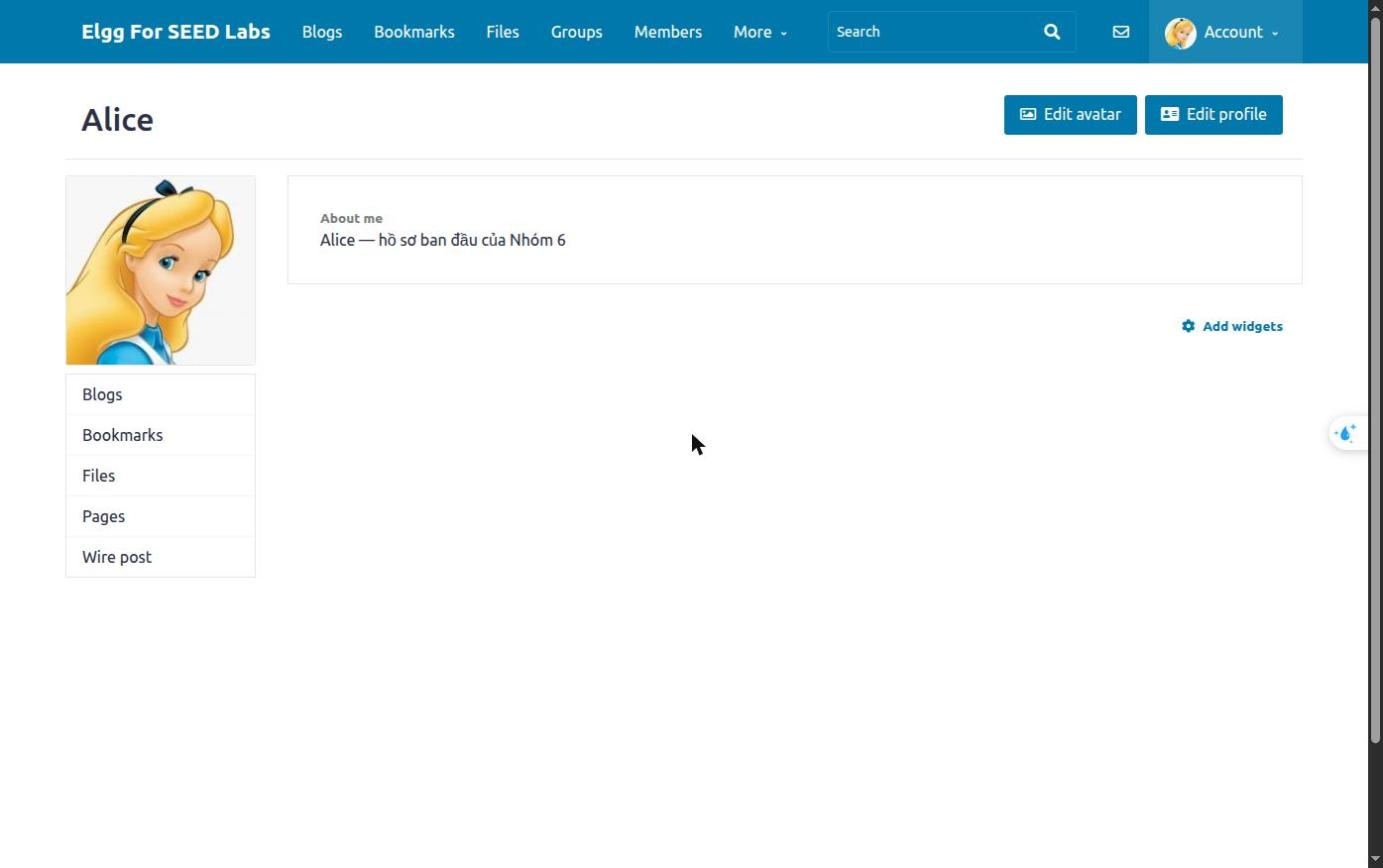
\includegraphics[width=\linewidth]{img/ev-before.jpg}
      \\[2pt]\scriptsize\textbf{Before:} baseline About me
    \column{0.34\textwidth}\centering
      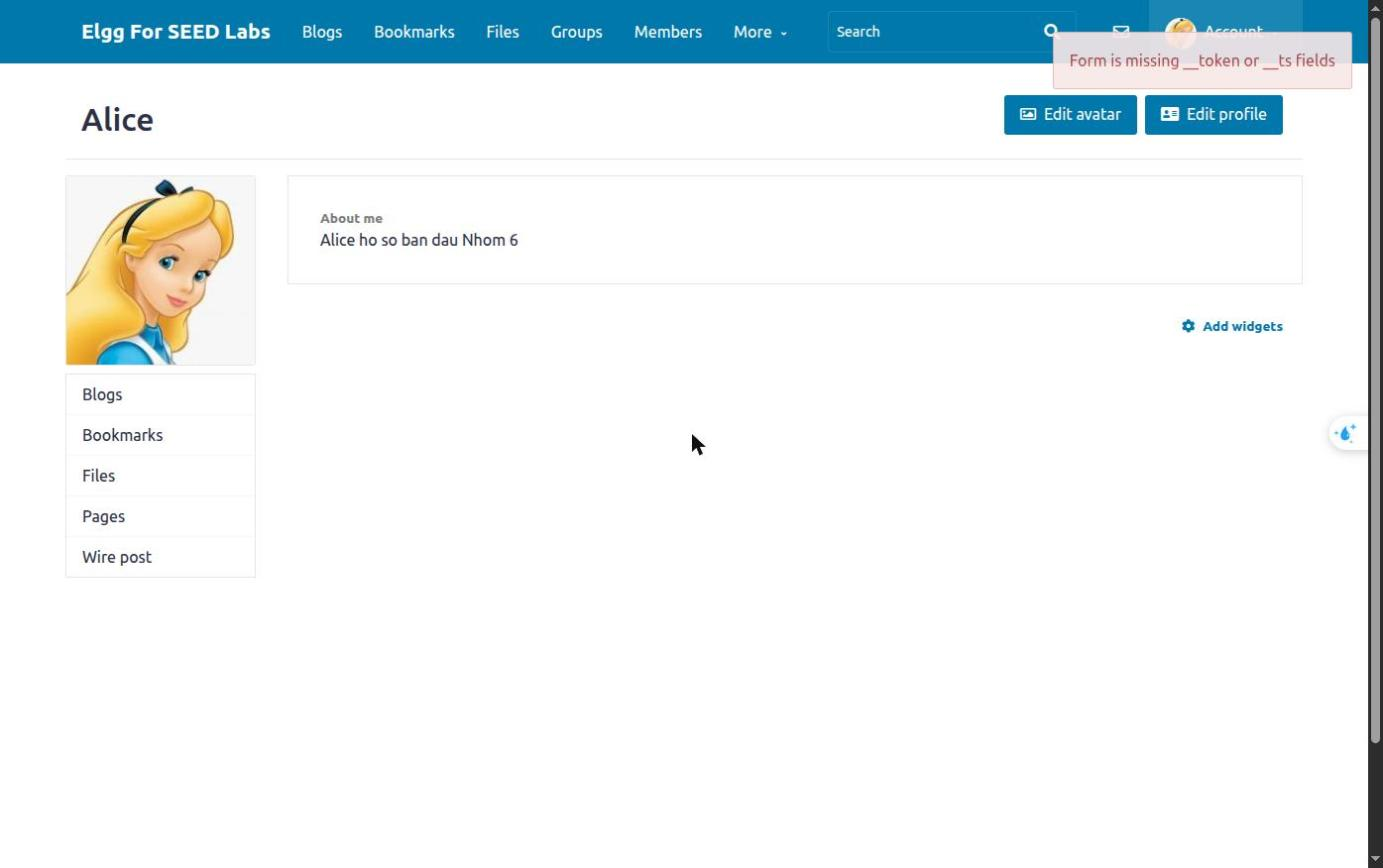
\includegraphics[width=\linewidth]{img/ev-protected-blocked.jpg}
      \\[2pt]\scriptsize\textbf{Protected:} \alert{``missing \_\_token''}
    \column{0.34\textwidth}\centering
      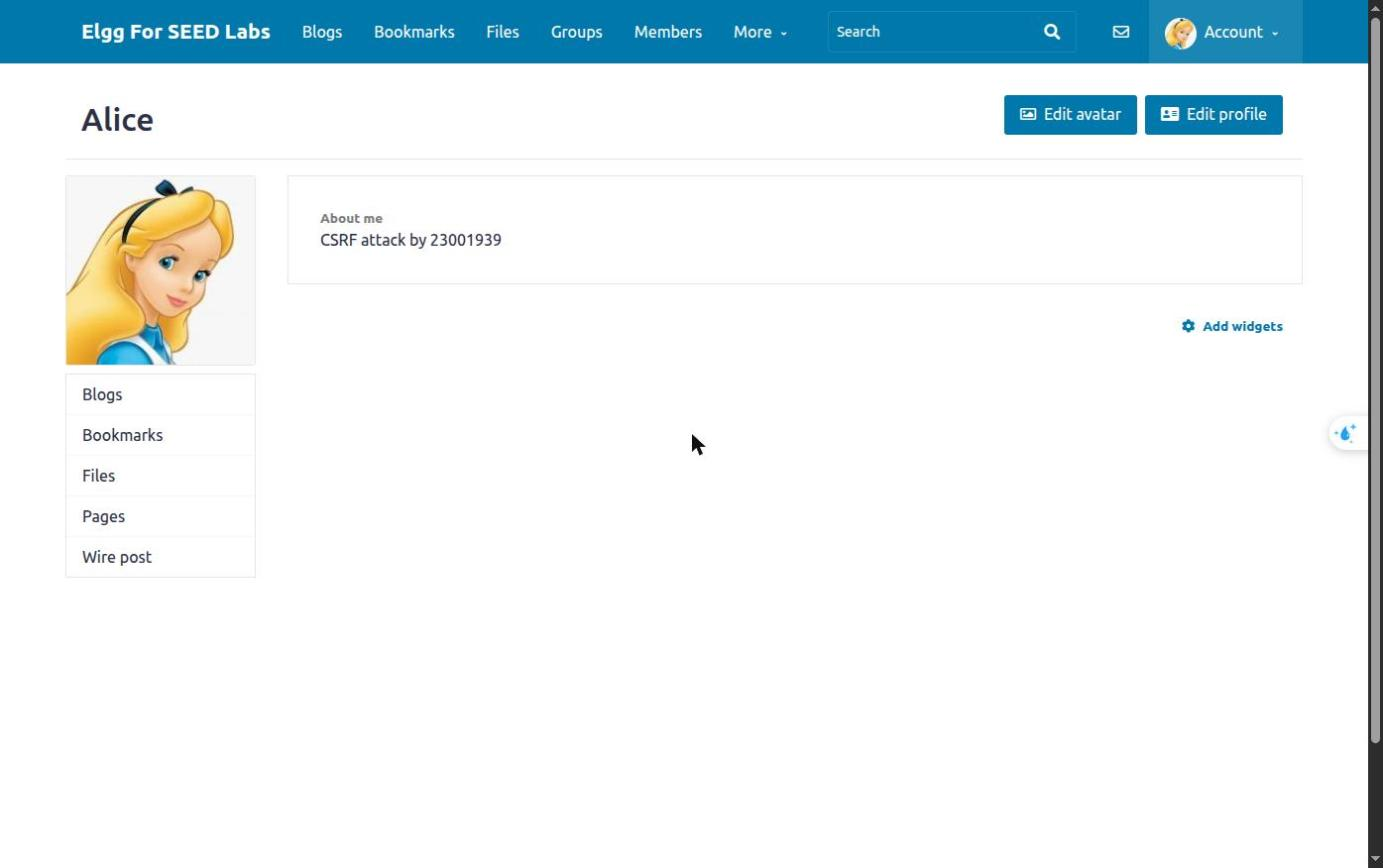
\includegraphics[width=\linewidth]{img/ev-after-success.jpg}
      \\[2pt]\scriptsize\textbf{After (vulnerable):} changed
  \end{columns}
  \vfill
  \begin{exampleblock}{Result matrix}
    \scriptsize
    \begin{tabular}{llcc}
      protected · same-site & token on & \textbf{blocked} & \no{} change\\
      vulnerable · cross-site & SameSite & \textbf{blocked} & \no{} change\\
      vulnerable · same-site & token off & \textbf{success} & \yes{} change\\
    \end{tabular}
  \end{exampleblock}
\end{frame}

\begin{frame}{Two defenses — proven independently}
  \footnotesize
  \begin{columns}[t]
    \column{0.5\textwidth}
      \begin{block}{Anti-CSRF token (server)}
        \scriptsize Attacker cannot read the token (SOP) $\Rightarrow$ forged request lacks it $\Rightarrow$ Elgg rejects: \alert{``Form is missing \_\_token''}.
      \end{block}
    \column{0.5\textwidth}
      \begin{block}{SameSite cookie (browser)}
        \scriptsize Even with the token off, a \emph{cross-site} POST carries no session cookie $\Rightarrow$ Elgg sees a stranger $\Rightarrow$ profile unchanged.
      \end{block}
  \end{columns}
  \vfill
  \begin{alertblock}{Technical finding}
    \scriptsize About me is stored as the \emph{annotation} \texttt{profile:description}, not the metadata \texttt{\$user->description} $\Rightarrow$ the \texttt{reset-profile} tool reset the wrong table. Lesson: trust only directly-verified evidence.
  \end{alertblock}
\end{frame}

\begin{frame}{Defense-in-Depth}
  \footnotesize
  \begin{tabular}{ll}
    \toprule
    \textbf{Layer} & \textbf{Measure}\\
    \midrule
    Cookie & \texttt{SameSite=Lax/Strict} — no cross-site cookie\\
    Application & Anti-CSRF token — attacker cannot read it (SOP)\\
    Application & Double Submit Cookie\\
    Header & Check \texttt{Origin} / \texttt{Sec-Fetch-Site}\\
    UI & \texttt{X-Frame-Options} / CSP \texttt{frame-ancestors}\\
    \bottomrule
  \end{tabular}
  \medskip
  \begin{block}{Recommendation}
    \footnotesize \texttt{SameSite=Lax} + anti-CSRF token + \texttt{Origin} check on sensitive endpoints. Never use \texttt{GET} for state-changing actions.
  \end{block}
\end{frame}

\begin{frame}{AI disclosure \& conclusion}
  \textbf{AI usage levels:}
  \begin{itemize}\small
    \item \textbf{Level 1:} discuss CORS/Simple Request mechanics — students write the code.
    \item \textbf{Level 2:} AI co-creates formatting/diagrams following the group's design.
    \item \textbf{Level 3:} AI helps scaffold tooling \& test automation; the group configures, runs, and owns the results.
  \end{itemize}
  \vfill
  \begin{alertblock}{Core message}
    \small CSRF is \textbf{not} stopped by HTTPS. The real fix: \texttt{SameSite} cookies + anti-CSRF tokens + request-origin checks. \textit{Learn to attack in order to defend.}
  \end{alertblock}
\end{frame}

{\setbeamercolor{background canvas}{bg=navy}
\begin{frame}[plain]
  \centering\vfill
  {\color{white}\Huge\textbf{Thank you!}}\\[10pt]
  {\color{mist}\large Questions \& Answers}
  \vfill
\end{frame}}

\end{document}
